In this section, we compare packet-based application prediction and flow unit application prediction.
CNN and ResNet are used for packet unit prediction.
RNN and LSTM are used for flow unit prediction.
In addition, we compare the performance of the model with the flow unit and the packet unit through the overall comparison of CNN, ResNet, RNN, and LSTM.

\subsection{Experiments Environment}
The learning model is based on CNN, RNN, and LSTM supported by Keras 2.2.0.
In case of ResNet, network model was constructed using CNN model supported by Keras.
Model learning epochs were set to 200.

In the experiments environment, we run the models on Ubuntu 16.04 LTS using 32GB of RAM and two GPU cards of which model is NVIDIA GTX 1080Ti 11GB.
Experiments implementation uses Tensorflow-gpu 1.8 and Keras 2.2.0 operated with Python 3.6.

The experiment performs Scikit-learn's GridSearchCV for one dataset and finds the optimal hyper-parameters through each model tuning.
The model learning was performed using optimal hyper-parameters for each dataset in Tables 1, 2, 3 and 4 of the Section.\ref{sec:modeltunning}.

\subsection{Performance Metrics}
In this paper, we use precision, recall, and f1-score \cite{citeulike:12882259} for performance comparison of CNN, ResNet, RNN and LSTM models.
Recall, precision, and f1-score provide performance metrics that take into account the unbalanced distribution of each application.
f1-score is the most important metric in all metrics.
f1-score represents the harmonic mean of precision and recall and represents the classification performance of unbalanced datasets.
The f1-score is expressed as 0 to 1 and is the best value at 1.

The definition of recall, precision and f1-score follows four previous definitions as follow:
First, False Positive (FP) indicates that the prediction is that the application is correct, but not actually the application.
Second, False Negative (FN) indicates that the application is not expecting the result, but the application is actually correct.
Third, True Positive (TP) indicates that the application is correct and the application is correct.
Finally, True Negative (TN) indicates that the application is not the result of the prediction, but is not actually the application.
The definition of recall, precision and f1-score according to the previous definition is as follows:

\begin{equation}
Recall =  \frac{TP}{TP + FP}
\end{equation}

\begin{equation}
Precision =  \frac{TP}{TP + FN}
\end{equation}

\begin{equation}
F1-score =  \frac{2 \times Precision \times Recall}{Precision + Recall}
\end{equation}

\subsection{Experiments Results}
The first experiment is a comparison of CNN and ResNet with the packet unit datasets.
In order to compare CNN and ResNet, the total f1-score was compared by varying the payload size of the packet to $6 \times 6 (36)$, $8 \times 8 (64)$, $16 \times 16 (256)$, and $32 \times 32 (1024)$.

\begin{figure}[t]
\centering
{
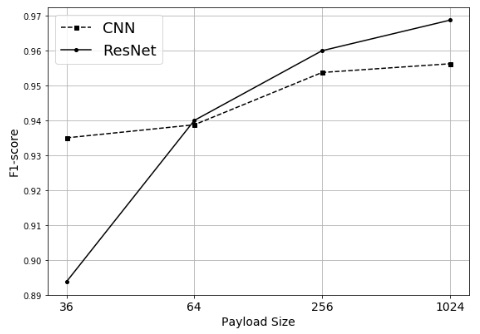
\includegraphics[width=3.4in]{fig7.jpg}
\caption{Comparison of CNN and ResNet with the overall f1-score for each application}
\label{fig7}
}
\end{figure}

Fig.\ref{fig7} compares f1-score for all applications by payload size in CNN and ResNet.
If the payload size of the packet is small, it can be seen that the overall f1-score value of CNN is about 0.4 higher than ResNet.
However, as the payload size increases, the training data set size also increases.
As a result, f1-score of ResNet is larger than CNN.
The reason is that because the learning model of ResNet is complex, less learning data sets are not good for learning.
Conversely, the larger the payload size and the larger the training data set, the better the performance of the more complicated ResNet model.

\begin{figure*}[h]
\centering
{
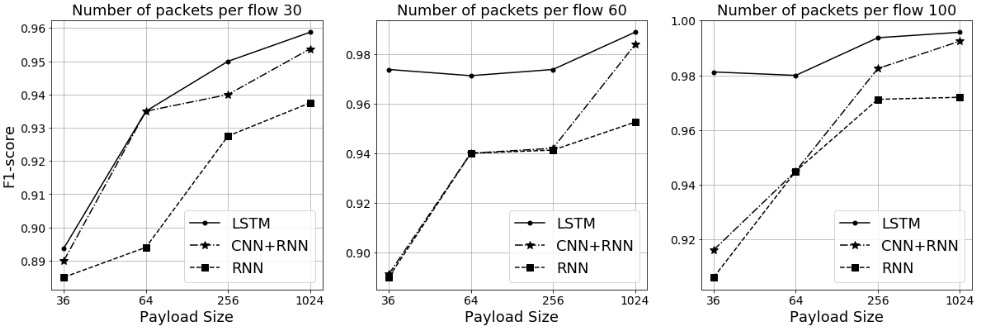
\includegraphics[scale=0.5]{fig9.jpg}
\caption{Comparison of RNN, LSTM and CNN+RNN with the overall f1-score for each application}
\label{fig9}
}
\end{figure*}

The following experiment is a comparison of RNN, LSTM, and CNN + RNN using flow unit datasets.
Fig.\ref{fig9} shows the total f1-score for each packet's payload size and the number of packets per flow.
It can be seen that the overall f1-score increases as the payload size of the packet increases.
Also, as the number of packets per flow increases, the entire f1-score increases.
When the number of packets per flow is 30 and the payload size is 36, the f1-score of each RNN, LSTM, and CNN + RNN is 0.885, 0.89375 and 0.89.
However, when the number of packets per flow is 100 and the payload size is 1024, each f1-score thereof is 0.972, 0.99575 and 0.9925.
It is noticed that the f1-score across LSTM is higher than the total F1-score RNN and CNN + RNN.
It indicates that LSTM alone can provide similar or better performance without using complex models in the flow unit learning model.

\begin{figure}[t]
\centering
{
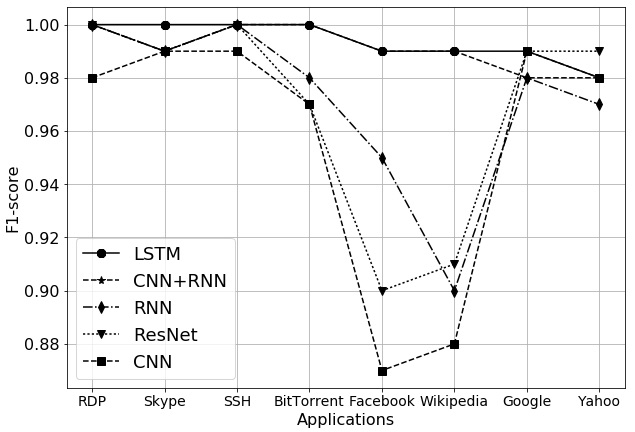
\includegraphics[width=3.3in]{fig10.jpg}
\caption{Comparison of packet unit classification and flow unit classification}
\label{fig10}
}
\end{figure}

Fig.\ref{fig10} is a graph comparing the f1-score results for each application when using a deep learning model to compare packet units and flow unit classifications.
In the case of CNN and ResNet, it represents the f1-score for each application when the payload size is $32 \times 32 (1024)$.
Also, in the case of RNN, LSTM, and CNN + RNN, it indicates the f1-score for each application when the payload size is 1024 and the number of packets per flow is 100.
Packet unit learning models CNN and ResNet show that f1-score on Facebook and Wikipedia are smaller than other applications.
The facebook and wikipedia packets are very similar to each other, so they are smaller than the f1-score of other applications' packets.
In the case of RNN, we can see that f1-score value of Facebook and Wikipedia are low as in the case of packet unit classification.
However, in the case of LSTM and CNN + RNN, the f1-score of both applications is high.
Thus, we can see that the LSTM and CNN + RNN learning models are well-categorized and that the LSTM performs better with subtle differences.